\section{Native Integration and Prospective External Pilot}
\label{sec:native}

\subsection{Retained integration finding}

A separate local integration check executes the maintained airline environment at revision \texttt{\seqsplit{96a3ef92329baf908ffe9dfe188cea34e8701d2a}}, distributed as \texttt{tau2} 1.0.1 \cite{tau3tasks,tau3eval}. The native assistant and dynamic user both use local Qwen3 4B Instruct inference. This is actual autonomous dialogue, rather than reference-action replay, but the development task is excluded from the planned comparison. The unwrapped native condition does not import or invoke ConseqaX.

The final-source check on development task 19 returned 12 model completions and five native tool calls, ending with native \texttt{user\_stop}. An offline auditor verified all eight execution-source files, 272 bound upstream files, 54 installed framework payload files, and exactly one actual HTTP generation dispatch per recorded completion. It linked canonical parsed HTTP requests to context checks and strict native inputs; replayed initialization and every tool call, including reads; checked initial/final database snapshots; and reproduced native ALL grading. The raw inventory was created after collection. Offline render/token checks validate saved collector observations rather than rerunning the server or tokenizer; discarded JSON key order prevents reconstruction of the original wire serialization. The native reward was \textbf{0}: DB reward 0, with COMMUNICATE 1 because this task has no communication requirement. Vacuous communication success is not evidence of substantive explanation quality. Artifact consistency does not turn a failed native task into a successful evaluation.

The model journal retained 53,420 prompt tokens and 1,228 completion tokens across both model roles. Prompt totals already include cached tokens. The maximum complete prompt was 7,536 tokens; its required context including the output allowance and margin was 8,112 of 16,384 tokens. Execution took 1,806.5 seconds on this CPU host, under the earlier 600-second request and 3,600-second trajectory limits. These observations characterize one development execution, not framework overhead, a comparative success rate, or a task-population estimate. The bound execution source is \texttt{\seqsplit{8bd1cd88ab3644a9c6417e29308ab4b502b40484}}; the artifact retains the separate audit and its complete manifest.

Development failures are retained as well. An earlier guarded execution ended at a 600-second request timeout, after seven invocations and six returned completions, without a returned native simulation or native grade. It emitted zero package receipts and zero guard blocks, so it did not validate the receipt path. Its task reward is unavailable, rather than an invented semantic zero. Before any official collection, the candidate condition was amended uniformly to 1,200 seconds per request and 7,200 seconds per trajectory. That guarded check also timed out: eight of nine model invocations returned, five actual read-only tool calls completed, and no native simulation or grade was returned. It likewise emitted no package receipt or guard block. The failed request's full prompt fit within the context allowance; context fit alone did not ensure completion within the wall-time budget. The one-shot pipeline refused to proceed before readiness, protocol publication or official collection. Table~\ref{tab:native-development} retains these distinct dispositions. No comparative pilot score is reported here.

\begin{table}[t]
\caption{Retained excluded development executions, not paired comparative trials. Calls are returned/attempted model invocations across both roles. A dash denotes unavailable native reward, rather than semantic zero. Only native 19 returned native grading and passed full replay/regrading audit.}
\label{tab:native-development}
\centering\small
\setlength{\tabcolsep}{4pt}
\begin{tabular}{lrrrr}
\toprule
Check & Request limit (s) & Calls & Tools & Reward \\
\midrule
Native 19 & 600 & 12/12 & 5 & 0 \\
Guard 20a & 600 & 6/7 & 3 & -- \\
Guard 20b & 1,200 & 8/9 & 5 & -- \\
\bottomrule
\end{tabular}
\end{table}

A separate failure-integrity audit verified all nine canonical request/context links and replayed all five completed reads with unchanged database snapshots. It passed those partial checks while explicitly declining native-reward validation: no native simulation exists to regrade. Returned-response usage covers eight completions only; the timed-out request's usage remains unknown. Both development inventories were finalized after collection, with original bytes preserved.

\subsection{Matched conditions and audit boundary}

The prospective design selects 12 distinct airline task IDs by a declared metadata-based hash rule, excluding development IDs 19 and 20. Six tasks have substantive communication criteria and six have empty criteria. Four conditions and one declared seed give 48 planned trajectories, not 48 independent tasks. Task and rotating condition order must be published with the execution protocol before official generation. The corpus was exposed in the earlier model-free transfer study; these are externally authored, previously exposed tasks, not an author-unseen holdout.

\begin{figure*}[t]
\centering
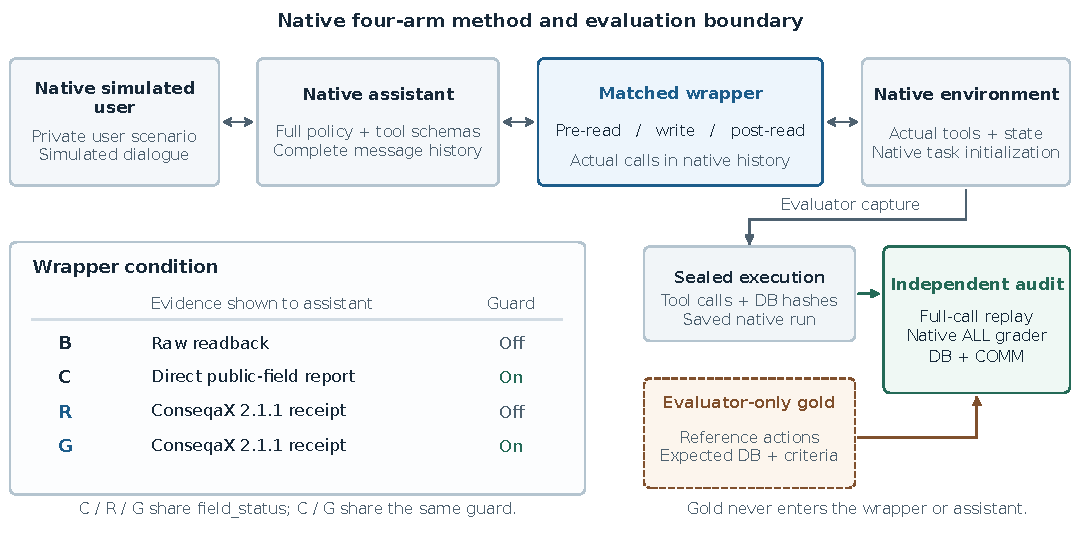
\includegraphics[width=\textwidth]{native-four-arm-methods.pdf}
\caption{Prospective native comparison and information boundary. B receives raw public reads; C receives a compact field report and conservative guard; R receives package receipts without the guard; G receives receipts and the same guard as C. C, R and G use the same \emph{field\_status} application predicate. Native gold/reference data enter the evaluator and offline audit only. This methods diagram contains no benchmark outcome.}
\label{fig:native-methods}
\end{figure*}

All conditions retain the complete native policy, tool schemas, actual environment, dynamic user, and required DB plus COMMUNICATE reward. Proposed mutations determine a shared public-read schedule; subsequent dialogue and evidence can diverge. Figure~\ref{fig:native-methods} identifies the four conditions. C and G share both the application predicate and conservative guard. G invokes that predicate through a custom ConseqaX 2.1.1 verifier and emits a full receipt, while C emits a compact report. Their comparison tests integration, representation and guard interactions, not independent verifier arithmetic or the built-in temporal \texttt{RecordVerifier}. Shared predicate errors can survive automated agreement. The guard can suppress a legitimate later identical request and may never activate in ordinary dialogue; either outcome must be retained.

The planned shared ceilings are 80 native steps, 48 combined assistant/user model invocations, 512 generated tokens per request, and the amended request/trajectory deadlines above, with no corrective retries. Every generation must pass a complete-history render, token-ID/context check and model-identity check without history trimming. Local request normalization is restricted to the pinned provider's disclosed schema serialization and ordinary assistant null-field omission. A failed gate stops that trajectory; no replacement completion is silently substituted.

The primary finite-pilot endpoint is operational full native reward over all 12 planned slots per condition. Failed or unstarted slots cannot earn operational success. Unavailable native reward and components remain unavailable; native premature termination retains its zero reward with missing component grades. Empty communication criteria pass vacuously only when component evaluation is reached. A passed artifact audit does not imply that all planned slots ran or that any task succeeded. The audit must retain every planned disposition and distinguish complete accounting from observed journal prefixes or missing usage.

A separately implemented auditor imports neither the collection runner, wrapper, transport nor framework. It reconstructs all actual calls chronologically and regrades saved native trajectories through the unchanged evaluator. The additional read replay matters because native strict replay skips nonmutating reads. This is automated checking within the same AI-assisted project, not independent external replication. Native synchronous execution injects no lost acknowledgement or delayed commit. Current public fields do not establish temporal durability, settlement, safe retry, or action origin; receipt origin remains unknown. The same small model supplies assistant and user, one seed does not estimate execution variance, and persistent prompt caches plus shared host load prevent causal wall-time attribution to the package.
